% Template for Cogsci submission with R Markdown

% Stuff changed from original Markdown PLOS Template
\documentclass[10pt, letterpaper]{article}

\usepackage{cogsci}
\usepackage{pslatex}
\usepackage{float}
\usepackage{caption}

% amsmath package, useful for mathematical formulas
\usepackage{amsmath}

% amssymb package, useful for mathematical symbols
\usepackage{amssymb}

% hyperref package, useful for hyperlinks
\usepackage{hyperref}

% graphicx package, useful for including eps and pdf graphics
% include graphics with the command \includegraphics
\usepackage{graphicx}

% Sweave(-like)
\usepackage{fancyvrb}
\DefineVerbatimEnvironment{Sinput}{Verbatim}{fontshape=sl}
\DefineVerbatimEnvironment{Soutput}{Verbatim}{}
\DefineVerbatimEnvironment{Scode}{Verbatim}{fontshape=sl}
\newenvironment{Schunk}{}{}
\DefineVerbatimEnvironment{Code}{Verbatim}{}
\DefineVerbatimEnvironment{CodeInput}{Verbatim}{fontshape=sl}
\DefineVerbatimEnvironment{CodeOutput}{Verbatim}{}
\newenvironment{CodeChunk}{}{}

% cite package, to clean up citations in the main text. Do not remove.
\usepackage{cite}

\usepackage{color}

% Use doublespacing - comment out for single spacing
%\usepackage{setspace}
%\doublespacing


% % Text layout
% \topmargin 0.0cm
% \oddsidemargin 0.5cm
% \evensidemargin 0.5cm
% \textwidth 16cm
% \textheight 21cm

\title{How should we structure learning contexts? Understanding the mix of
active and passive learning}


\author{{\large \bf Kyle MacDonald} \\ \texttt{kyle.macdonald@university.edu} \\ Department of Psychology \\ Stanford University \And {\large \bf Michael C. Frank} \\ \texttt{mcfrank@university.edu} \\ Department of Psychology \\ Stanford University}

\begin{document}

\maketitle

\begin{abstract}
Much of what we know depends on contexts that contain \emph{both} active
and passive learning. But how should we structure the environment in
order to maximize learning outcomes? In the current work, we explore how
different sequences of active and passive training affect concept
learning in adults. First, we replicate the active over passive learning
advantage found in Markant \& Gureckis (2014) (Experiments 1a and 1b).
Then in Experiment 2, we provide a direct test of how different
sequences of active/passive training affect people's learning outcomes.
Across both experiments, active training leads to better overall
learning of the target concept compared to passive training.
Interestingly, in Experiment 2 ``passive-first'' learners performed
better than ``active-first'' learners. These data provide evidence that
active learning can be more effective after people have constructed a
stronger representation of the learning task.

\textbf{Keywords:}
self-directed learning, concept learning, replication
\end{abstract}

\section{Introduction}\label{introduction}

Learning is the result of a complex interaction of active and passive
processes. It is almost impossible to think of a case where people learn
a concept entirely from information that they generate themselves
(active learning) or entirely from information generated from the world
(passive learning). And yet we know relatively little about how to best
structure the sequence of active and passive learning in order to
maximize learning outcomes. For example, consider a teacher introducing
a challenging math concept: should she allow students to explore first
and then provide instruction, or should she teach first and then let
students actively explore?

The potential advantage for active learning has been the focus of
research in education (Grabinger \& Dunlap, 1995), machine learning
(Settles, 2012), and cognitive science (Castro et al., 2009). In the
majority of these studies, researchers isolate active and passive
training, and test which regime leads to better learning outcomes. In
their review of this literature, Gureckis \& Markant (2012) present a
set a general ``cognitive'' explanations for why active learning might
be helpful across different tasks and learning contexts. One explanation
is that people can use their prior experience to select the most
informative examples (e.g., asking a question about something that is
particularly confusing). Another explanation is that the process of
active learning causes people to engage more deeply with the task,
allowing them to develop better learning strategies.\footnote{This idea
  is similar to work showing that simply providing an explanation can
  deepen understanding of a concept (Lombrozo, 2006).} But Gureckis \&
Markant (2012) point out that the effectiveness of selection-based
learning is fundamentally linked to the quality of the learner's
\emph{representation of the task}. If the representation is poor, or
there is a prior misconception, then active learning will not be
effective and might even lead to biased information seeking (e.g.,
confirmation bias (Nickerson, 1998)).

These cognitive explanations lead to competing predictions about the
effectiveness of different sequences of active and passive learning. One
prediction is that receiving active learning first (active-first) is
better because it engages learners and allows them to develop better
learning strategies. Research from education on the concept of
\emph{Productive Failure} shows that allowing students to first struggle
(typically in the form of self-directed problem solving) with a task,
leads to better uptake of subsequent instruction (Westermann \& Rummel,
2012). Moreover, in a tightly controlled cross-situational word learning
task, Kachergis, Yu, \& Shiffrin (2013) found that people who received
active learning first preformed better overall when asked to recall
newly learned words. Kachergis et al. (2013) suggest that learners
developed better attentional and memory strategies during the active
training, which transferred to passive learning context, increasing
overall acccuracy.

The competing prediction is that receiving passive learning first
(passive-first) is better because it helps to set up a stronger task
representation, allowing people to use their subsequent active learning
more effectively. Evidence in support of this prediction comes from
research that explores the contexts when the active learning advantage
breaks down. For example, in a category learning task, Markant \&
Gureckis (2014) found that active learning provided no benefit over
passive learning when the target category structure was different from
people's prior expectations. They suggest that the separation between
expectation and concept caused people to select less helpful examples.
In addition, work from machine learning shows that in practical settings
random sampling is preferable to active learning when the correct model
class (i.e., representation of the task) is unknown (Settles, 2012).

\begin{CodeChunk}
\captionsetup{width=0.8\textwidth}\begin{figure*}[t]

{\centering 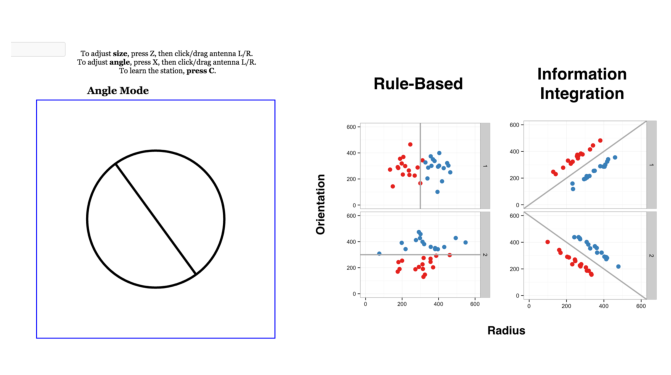
\includegraphics{figs/stimuli_exp1-1} 

}

\caption[The left panel shows a screenshot of the stimuli used in Experiments 1 and 2]{The left panel shows a screenshot of the stimuli used in Experiments 1 and 2. The right panel shows examples of distributions of training stimuli shown to participants in the passive learning condition. Each point represents a different antenna, constructed with an orientation value (vertical axis) and radius value (horizontal axis). The color of the points show the category membership of each antenna (red is Channel 1, blue is Channel 2). The solid line in each facet represents  the optimal category boundary for both the Rule-Based category and the Information-Integration category structures.}\label{fig:stimuli_exp1}
\end{figure*}
\end{CodeChunk}

In the current work, we set out to test these two predictions by
exploring the effectiveness of different sequences of active/passive
learning. We use a category learning paradigm from Markant \& Gureckis
(2014), where they found a reliable advantage for active over passive
learning. In this task, people learn one of two abstract categories: a
Rule-Based (RB) structure where the category boundary varied along a
single dimension (e.g., size), and a more complex
Information-Integration (II) structure where the category boundary was
defined by two dimensions (e.g., size and angle). Active learners
generate their own examples to test their beliefs; whereas passive
learners receive examples that were generated randomly.

We predicted that passive-first training would be better in this task
because learners can generate and refine hypotheses during the passive
block, which they then refine with highly informative examples in the
active block. Moreover, Markant \& Gureckis (2014) found that the
quality of sampling behavior was ``worse than random in the early blocks
of their experiment, suggesting that active learning was less effective
early in the task.

The plan of the paper is as follows: In Experiments 1a, we present a
direct replication of the active learning advantage found in Markant \&
Gureckis (2014) for the RB category structure. In Experiment 1b, we test
the more complex II category structure. Then, in Experiment 2, we build
on our replication data to show that passive-first training is more
effective compared to active-first training. Together, the data suggest
that active learning can provide an advantage over passive learning, but
this advantage depends on the learner's representation of the task,
which can be improved by receiving more experience with the task.

\section{Experiment 1a}\label{experiment-1a}

Experiment 1a is a direct replication of the advantage for active
learning over passive learning found in Markant \& Gureckis (2014). We
tested participants' category learning for the RB category structure
after receiving either active or passive training. We used the same
stimuli and followed the exact procedures as the original study
(described below). All of the stimuli and the experiments can be viewed
and downloaded at the project page for this paper:
\url{https://kemacdonald.github.io/Act-Learn/}.

\begin{CodeChunk}
\captionsetup{width=0.8\textwidth}\begin{figure*}[t]

{\centering 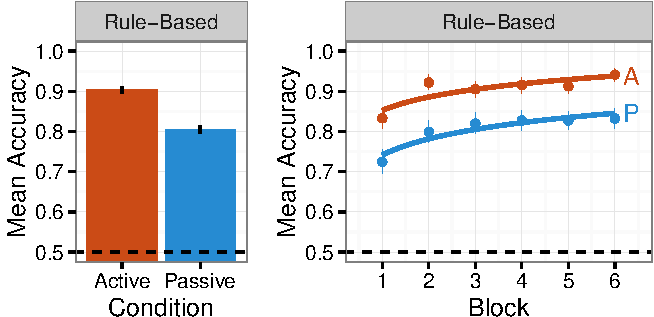
\includegraphics{figs/exp1a_acc_plot-1} 

}

\caption[The left panel shows overall accuracy performance for the Active and Passive training conditions]{The left panel shows overall accuracy performance for the Active and Passive training conditions. The right panel shows participants' accuracy across each of the six blocks in the experiment. Colored lines are generated by a binomial smoother and error bars indicate 95\% confidence intervals computed by non-parametric bootstrap.}\label{fig:exp1a_acc_plot}
\end{figure*}
\end{CodeChunk}

\subsection{Methods}\label{methods}

\subsubsection{Power analysis and planned
sample}\label{power-analysis-and-planned-sample}

We calculated Cohen's d for the test comparing overall accuracy between
the active and passive learning conditions (d = 0.47). Next we conducted
a post hoc power analysis and found that the original study achieved a
power of \%43. Finally, we conducted an a priori power analysis for the
proposed replication in order to achieve 80\%, 90\%, and 95\% power to
detect that effect size. The results were: 80\% (n = 84, 42 in each
group), 90\% (n = 158, 79 in each group), and 95\% (n = 238, 119 in each
group). Our planned sample size was 48 participants, 24 in each
condition. This sample size allowed us to achieve 47\% power to detect
the an effect the size of the original finding. This sample size was
chosen to maximize power within our funding constraints.

\subsubsection{Participants}\label{participants}

We posted a set of Human Intelligence Tasks (HITs) to Amazon Mechanical
Turk. Only participants with US IP addresses and a task approval rate
above 85\% were allowed to participate, and each HIT paid one dollar.
Approximately 25 HITs were posted for each of the two between-subjects
conditions. Data were excluded if participants completed the task more
than once or if they reported that they did not understand the task at
the end of the experiment (1 HITs). The final sample consisted of 52
participants.

\subsubsection{Stimuli}\label{stimuli}

The left panel of Figure 1 shows a screenshot of the stimuli used in
across all experiments. Visual stimuli were black ``antennas'' on a
white background. Each antenna could vary along two continuous
dimensions -- radius size or central angle -- and was assigned a value
between 1 and 600. These values were converted to pixel values for
display on a computer screen. To ensure that participants could not
complete a full rotation of the antenna, the rotation of the central
angle was limited to 150 degrees. The minimum radius and angle values
were randomized for each participant, such that each participant was
assigned a unique optimal decision boundary. Finally, we used a
Rule-Based category structure where the category boundary is defined
along a single dimension: either the antenna's size or central angle
(see the right panel of Figure 1).

Radius and angle values for the 96 passive training trials were
generated from two Gaussian distributions with identical mean and
covariance parameters as Markant \& Gureckis (2014) (see the right panel
of Figure 1). For test trials, we created a uniform grid of 192 unique
test items that covered the entire feature space. We randomly sampled 8
items from each quadrant to get 32 test trials for each block. We then
randomized the order of the training and test trials within each block
for each participant.

\subsubsection{Design and procedure}\label{design-and-procedure}

Participants saw a total of 288 trials (96 training trials and 192 test
trials) across 6 blocks. Each block consisted of 16 training trials and
32 test trials. Before starting the task, participants were told that
this was a game where they would see ``loop antennas'' for televisions
and each antenna received one of two channels (CH1 or CH2), and their
goal was to learn the difference between the two types of antennas. We
introduced some uncertainty by telling participants that the antennas
could pick up the wrong channel on occasion, and that they should learn
what channel is most often received by a particular type of antenna.

After the instructions, participants were randomly assigned to one the
two between-subjects conditions (Active vs.~Passive training). In the
Active training condition, participants were able to design their own
antennas to test. They modified the antenna by clicking and dragging the
mouse from left to right. To change the size of the antenna, they first
pressed the ``Z'' key. To change the angle, they first pressed the ``X''
key. When participants were finished with their design, they pressed the
spacebar to see which channel (Ch1 or Ch2) the antenna received. The
channel label appeared in a text box with a green border located above
the antenna.

In the Passive training condition, participants were shown antennas with
size and angles generated from the underlying category distributions.
After a two second delay they were told which channel the antenna
received. To ensure that participants saw the channel, they had to click
on the channel text in order to advance the experiment. When they
clicked the channel text, a green box appeared around the text to
indicate that their response had been recorded.

After completing the training, participants in both conditions proceeded
to the test trials. On each test trial participants saw an antenna and
were asked, ``Which channel does this antenna receive?'' To indicate
their response participants selected one of two buttons located above
the antenna. At the end of each block of test trials, participants saw a
summary of their accuracy on the preceding block.

\subsection{Results and Discussion}\label{results-and-discussion}

\subsubsection{Overall classification
accuracy}\label{overall-classification-accuracy}

We directly followed the analysis plan of Markant \& Gureckis (2014),
using a t-test to compare overall test performance for participants in
the active and the passive learning conditions.
\footnote{All of our data, processing, and analysis code can be viewed in the version control repository for this paper at: https://github.com/kemacdonald/act-learn.}
The left panel of Figure 2 shows overall test performance, with active
learners being more accurate than passive learners, \(t\)(51) = 2.52,
\(p\) = 0.015.

\subsubsection{Classification accuracy across
blocks}\label{classification-accuracy-across-blocks}

The right panel of Figure 2 shows participants' accuracies across blocks
in the experiment. To quantify participants' behavior, we use mixed
effects regression models with the maximal random effects structure
justified by our experimental design: by-subject intercepts. We fit a
logistic regression predicting test performance based on condition
(active/passive) and block. The model was specified as
\texttt{Correct $\sim$ 1 + Condition * Block + (1 | subject)}. We found
a significant main effect of condition (\(\beta\) = -0.72, p \textless{}
.001) with better performance for active learners, and a significant
main effect of block (\(\beta\) = 0.19, p \textless{} .001) such that
responses were more accurate later in the experiment.

\subsubsection{Relationship between sampling behavior and
learning}\label{relationship-between-sampling-behavior-and-learning}

We were also interested in the relationship between participants'
overall sampling behavior and learning outcomes. We follow Markant \&
Gureckis (2014) and quantify the quality of a sample based on its
orthogonal distance from the true category boundary, with samples closer
to the boundary being of higher quality. For each participant, we
computed a mean accuracy score and a mean sample distance score, and fit
a linear model using sample distance to predict accuracy. We found a
signficant effect of sample distance (\(\beta\) = -.0003, p \textless{}
.001) with accuracy increasing as mean sample distance decreased.

Taken together, our data provide strong evidence for a successful
replication of the original results reported in Markant \& Gureckis
(2014). We found a comparable advantage in overall classification
accuracy for active learners over receptive learners in a web-based
experiment with two fewer training/test trial blocks. Our results differ
from the original study in that we found an immediate advantage for
active learners after the first block that was not present in the
original study. Next we attempt to replicate Markant \& Gureckis
(2014)'s findings for the II category structure and for the yoked
passive learning condition.

\section{Experiment 1b}\label{experiment-1b}

The goals of Experiment 1b are to (a) replicate Markant \& Gureckis
(2014)`s findings for the more difficult Information-Integration (II)
category structure, and (b) replicate the finding that passive learners
did not benefit from being ``yoked'' to active learners'
data.\footnote{Yoked designs are important because they help dissociate the effects of selection from the effects of seeing better data.}
They did not find an active learning advantage for the II category
structure and yoked learners were worse than active learners even though
they had seen the exact same learning information. We used the same
stimuli and followed the exact procedures as the original study
(described below). However, we reduced the length of the experiment to
two blocks. We made this decision based on finding an immediate active
learning advantage in Experiment 1a.

\subsection{Methods}\label{methods-1}

\subsubsection{Stimuli}\label{stimuli-1}

Visual stimuli were identical to Experiment 1a.

\subsubsection{Participants}\label{participants-1}

Participant recruitment and inclusionary/exclusionary criteria were
identical to those of Experiment 1a (excluded No, 3 HITs). 196 HITs were
posted across each of the between-subjects conditions: two category
structures (II and RB) and three training conditions (Active, Passive,
and Yoked).

\subsubsection{Design and procedure}\label{design-and-procedure-1}

Procedures were identical to those of Experiment 1a. We added a
``yoked'' learning condition, in which we match each passive learning
participant with training data generated from an active learning
participant's sampling behavior. Thus, both the active and yoked
participants saw the exact same data, but the active participants were
in control of the information flow.

\subsection{Results and Discussion}\label{results-and-discussion-1}

\subsubsection{Overall classification
accuracy}\label{overall-classification-accuracy-1}

\begin{CodeChunk}
\captionsetup{width=0.8\columnwidth}\begin{figure}[t]

{\centering 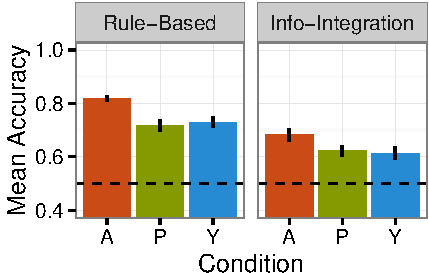
\includegraphics{figs/rep1b-acc-plot-1} 

}

\caption[The left panel shows overall accuracy performance for the Active and Passive training conditions]{The left panel shows overall accuracy performance for the Active and Passive training conditions. The right panel shows participants' accuracy across both blocks in the experiment.}\label{fig:rep1b-acc-plot}
\end{figure}
\end{CodeChunk}

Figure 3 shows the overall effect of category structure and training
condition on participants' accuracy performance. We fit the same
logistic regression as specified in Experiment 1a. We found a
significant main effect of category structure (\(\beta\) = -0.96, p
\textless{} .001) with better performance in the RB category structure,
and a significant main effect of condition (\(\beta\) = -0.72, p
\textless{} .001) such that participants in the passive and yoked
conditions performed worse than participants in the active condition. We
did not find any significant interactions.

\subsubsection{Relationship between sampling and test across
blocks}\label{relationship-between-sampling-and-test-across-blocks}

Since the main goal of this work was to test different sequences of
active/passive learning, we were interested in exploring the relations
between participants' sampling behavior and test accuracy \emph{over
time} in this task. To explore these relations, we performed an
exploratory analysis where we fit a linear model predicting each
participant's mean accuracy based on the quality of their sampling
behavior and block. As expected participants' accuracy improved in the
second block (\(\beta\) = 0.21, p = 0.01). There was a significant
two-way interaction between sampling distance and block (\(\beta\) =
-0.0013, p = 0.01) such that the relationship between quality of
sampling and accuracy did not emerge until the second block. Figure 4
shows this interaction.

TODO: quick recap and then transition to Experiment 2.

\begin{CodeChunk}
\captionsetup{width=0.8\columnwidth}\begin{figure}[h]

{\centering 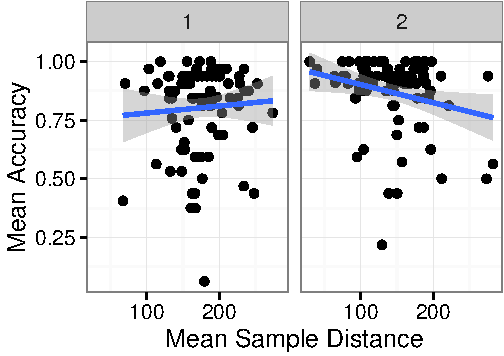
\includegraphics{figs/exp1_sampling-acc-plot-1} 

}

\caption[The relations between quality of sampling and accuracy on test trials across blocks]{The relations between quality of sampling and accuracy on test trials across blocks.}\label{fig:exp1_sampling-acc-plot}
\end{figure}
\end{CodeChunk}

\section{Experiment 2}\label{experiment-2}

TODO: introduce experiment 2.

\subsection{Methods}\label{methods-2}

\subsubsection{Stimuli}\label{stimuli-2}

Stimuli were identical to Experiment 1.

\subsubsection{Participants}\label{participants-2}

Participant recruitment and inclusionary/exclusionary criteria were
identical to those of Experiment 1 (No, 3 HITs). Approximately 44 HITs
were posted for each condition for total of 176 paid HITs.

\subsubsection{Design and procedure}\label{design-and-procedure-2}

Procedures were identical to those of Experiment 1. Participants were
randomly assigned to one the two between-subjects conditions:
Active-Receptive (AR) vs.~Receptive-Active (RA). In the AR condition,
participants completed a block of active learning then proceeded to a
block of passive learning. In the RA condition, the order of the blocks
was flipped.

\subsection{Results and Discussion}\label{results-and-discussion-2}

\begin{CodeChunk}
\captionsetup{width=0.8\textwidth}\begin{figure*}[t]

{\centering 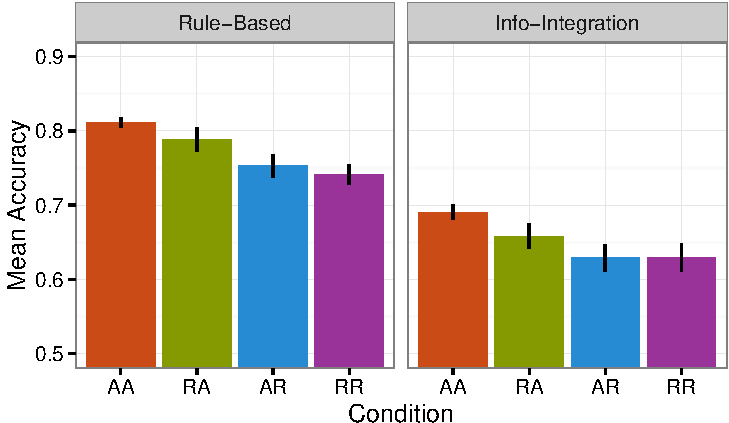
\includegraphics{figs/exp2_acc_plot-1} 

}

\caption[The left panel shows accuracy performance across both blocks for the different sequence of active/passive training]{The left panel shows accuracy performance across both blocks for the different sequence of active/passive training. The right panel shows overall accuracy performance plotted with the active-active and receptive-receptive data from Experiment 1.}\label{fig:exp2_acc_plot}
\end{figure*}
\end{CodeChunk}

Intercept is the mean of the means (or the grand mean) of all the
groups. These data are unbalanced. Active better than passive.
Information integration worse than rule-based.

\section{General Discussion}\label{general-discussion}

\begin{itemize}
\itemsep1pt\parskip0pt\parsep0pt
\item
  Recap findings

  \begin{itemize}
  \itemsep1pt\parskip0pt\parsep0pt
  \item
    Active learning advantage in a direct replication
  \item
    Passive-active better than Active-passive
  \item
    Conceptual replication
  \end{itemize}
\item
  Expand on why we see AR \textgreater{} RA

  \begin{itemize}
  \itemsep1pt\parskip0pt\parsep0pt
  \item
    Sequential hypothesis testing model
  \item
    Gain some understanding of task before exploring
  \item
    RA is bad because you can't refine your current hypothesis. Can only
    use the data you are given to confirm/reject current hypothesis
  \end{itemize}
\end{itemize}

Moreover, there are markedly different costs associated with active
compared to passive learning, with active learning requiring more effort
and time on the part of the learner. Thus, understanding how different
sequences of active/passive learning interact to affect learning
outcomes is an important question for both theoretical and applied
reasons.

\begin{itemize}
\itemsep1pt\parskip0pt\parsep0pt
\item
  Limitations

  \begin{itemize}
  \itemsep1pt\parskip0pt\parsep0pt
  \item
    AA was always best
  \item
    task analysis
  \item
    complexity of real world learning
  \end{itemize}
\item
  Takeaway point:
\end{itemize}

\section{Acknowledgements}\label{acknowledgements}

We are grateful to Doug Markant and Todd Gureckis for sharing the
details and code from the original experiment. We thank the members of
the Language and Cognition Lab for their helpful feedback on this
project. This work was supported by a National Science Foundation
Graduate Research Fellowship to KM.

\section{References}\label{references}

\setlength{\parindent}{-0.1in} \setlength{\leftskip}{0.125in} \noindent

Castro, R. M., Kalish, C., Nowak, R., Qian, R., Rogers, T., \& Zhu, X.
(2009). Human active learning. In \emph{Advances in neural information
processing systems} (pp. 241--248).

Grabinger, R. S., \& Dunlap, J. C. (1995). Rich environments for active
learning: A definition. \emph{Research in Learning Technology},
\emph{3}(2).

Gureckis, T. M., \& Markant, D. B. (2012). Self-directed learning a
cognitive and computational perspective. \emph{Perspectives on
Psychological Science}, \emph{7}(5), 464--481.

Kachergis, G., Yu, C., \& Shiffrin, R. M. (2013). Actively learning
object names across ambiguous situations. \emph{Topics in Cognitive
Science}, \emph{5}(1), 200--213.

Lombrozo, T. (2006). The structure and function of explanations.
\emph{Trends in Cognitive Sciences}, \emph{10}(10), 464--470.

Markant, D. B., \& Gureckis, T. M. (2014). Is it better to select or to
receive? Learning via active and passive hypothesis testing.
\emph{Journal of Experimental Psychology: General}, \emph{143}(1), 94.

Nickerson, R. S. (1998). Confirmation bias: A ubiquitous phenomenon in
many guises. \emph{Review of General Psychology}, \emph{2}(2), 175.

Settles, B. (2012). Active learning. \emph{Synthesis Lectures on
Artificial Intelligence and Machine Learning}, \emph{6}(1), 1--114.

Westermann, K., \& Rummel, N. (2012). Delaying instruction: Evidence
from a study in a university relearning setting. \emph{Instructional
Science}, \emph{40}(4), 673--689.

\end{document}
